\chapter{Dialog systems}
\label{ch:dialog-systems}

   
\section{Introduction}

\begin{quotation}\noindent
  I'm sorry, Dave, I'm afraid I can't do that.\\{} [Hal 9000, in Stanley
  Kubrick's 1968 film \mediatitle{2001: A Space Odyssey}, based on the book by Arthur C. Clarke]
\end{quotation}
\index{Kubrick, Stanley}
\index{Hal 9000 (evil computer)}
\index{Clarke, Arthur C.}



In the film \mediatitle{2001}, Hal is a computer that can use and
understand human language as well as we can.  The problem in the movie is that Hal becomes
so intelligent and independent that ``he'' starts disobeying Dave's commands.

We recommend that you pull up this scene on YouTube and watch it yourself.  Dave, the human astronaut, is stuck in a little spaceship pod, whereas Hal, the glowing red computer with a deadpan voice, controls the mothership.  Dave is ordering Hal to open the doors of the mothership so that he can come back inside; stuck in his little pod, he can't complete his mission and will eventually run out of air, water, and food.  Hal explains that he has figured out (by reading Dave's lips during a previous conversation with another astronaut) that Dave plans to shut him off, and declines to open the doors (\exsent{I'm sorry, Dave, I'm afraid I can't do that}) in order to save himself.  Dave says he'll go in through the emergency airlock, but Hal notes that Dave can't do that safely without his helmet, which Dave left inside the mothership.  As Dave becomes increasingly frustrated and frightened,  Hal calmly informs him that the conversation has become pointless.  The scene ends with Dave stuck outside in his pod, shouting at Hal, who has stopped responding.


This scene is famous for Kubrick's creepy, suspenseful style, but also for the questions that it raises about language technology.  It is discussed in the first pages of the classic NLP textbook by \citet{Jurafsky.Martin-09}  as a fictional example of a computer that has achieved human-level skills in conversation and reasoning, to which existing systems can be compared.  

Taking inspiration from their discussion, we can ask: What does Hal need to know -- about language, Dave, and the wider world -- in order to act as he does?  To understand what Dave is saying, Hal needs to know how to map speech to text, segmenting a continuous stream of sounds into words; he needs to know how to map text into structured sentences and how to understand their meaning.  To reply to Dave, he also needs to know how to map an idea into words, sentences, and ultimately speech.   He needs to understand the physical environment (the position of the pod, the doors, Dave, the helmet).  He needs to know how conversations work: when it is his turn to listen, how to update his representation of the world and of Dave's intentions based on what Dave says; when it is his turn to speak, how Dave's knowledge and intentions are in turn updated by what Hal says.    Hal  needs to know some conventions of politeness, for example when he (insincerely) softens his refusal with \exsent{I'm sorry} and \exsent{I'm afraid I can't}. And he needs meta-conversational knowledge about the purpose of the conversation, which he mentions explicitly when he unilaterally ends it.

To decide what to say and do, Hal needs to reason about different plans and possibilities for the future, as shaped by the actions of Dave and himself.  He needs to know that Dave intends to shut him off (which required him to read Dave's lips); that this is bad for Hal; and that Dave's plans can be subverted by keeping Dave outside the mothership (since Dave can only shut off Hal from inside).  In other words, Hal needs to understand his own goals, Dave's goals, and the conflict between them, as well as the pre-conditions and results of various potential events.


We can also ask: To what extent do modern systems measure up to the intelligence that these 1968 filmmakers imagined would be available in the year 2001 -- to what extent does life imitate art?  In some areas, such as text-to-speech, modern systems are pretty close to Hal.  In other areas, they are nowhere close: they aren't as good at reasoning about different people's goals and potential future events; they do not have Hal's capacity for (villainous) self-direction.  In addition to providing a fictional point of comparison for modern systems, 
Hal represents their potential for harm -- a theme that echoes throughout this book.

% talk more about this scene....
% chatbots versus dialog agents.... make this distinction clearer.
% Mitsuku, ELIZA, Hal, Siri...
% why are they female?

In computer science and linguistics, systems that ``converse'' like Hal are usually called \keyword{chatbots} when they are designed 
mainly for entertainment, providing chit-chat and keeping the conversation going any way they can (\exsent{Hi, what have you been up to?}), and \keyword{dialog agents} or \keyword{digital assistants} when they are designed to help the user achieve specific goals (such as booking appointments, setting alarms, or requesting directions).   The distinction is not always clear-cut (and people sometimes use these terms interchangeably), since digital assistants often need to show some social sensitivity,
and chatbots can combine chit-chat with specific goals such as providing mental health support or helping people practice their job interview skills.
As a fully versatile human-like character, Hal is partly a digital assistant (when ``he'' chooses to assist) and partly a chatbot.   
But at the level of the system's primary goals, a typical chatbot is built to resemble a social acquaintance, while a digital assistant is built to emulate a customer-service worker. 

The goal of this chapter is to give you the conceptual tools for understanding  and evaluating such systems. Since the first edition of this book (written in 2012), these systems have exploded in popularity and been woven into many other areas of language technology, such as writers' aids (\chapref{ch:writers-aids}) and search (\chapref{ch:searching}).

In this chapter, we describe how  conversations work between humans: how people exchange information, take turns speaking and listening, manage their social relationships, and what they implicitly assume about their conversation partner.   We explain why people build chatbots, how to build one, and how to evaluate whether it is doing a good job. Finally,  we explain why people build digital assistants, how to build one, and how to evaluate it.
  %  \item We will describe some of the things that people do when they talk to each other. We will focus mainly on situations where people are talking order to get something done, rather than on talk for the sake of talk.
   % \item We will describe the technology behind current (2020) digital assistants. We think this technology is well-designed and effective, but  does not remotely live up to the hype that it currently attracts.
%    \item We will describe what digital assistants do well and what do they do badly. There are direct and obvious measures of performance, especially when 
%    the task of the assistant is clear.
%    \item We will describe some user studies: what do people actually use digital assistants for? Also, not unrelated. what do users feel about them?     We will see that users generally like the assistants, but also report a lot of frustration.
%    \item We will talk a little about systems that are designed not to be effective but to be entertaining and engaging. These systems are   evaluated more on impressions and emotional connection than on performance.
%    \item We conclude with advice to anyone who is considering whether they or their business might want to deploy a digital assistant.   We suggest that if you are clear about exactly what the system is supposed to do, and that goal is not impossibly ambitious,     you will be able to choose an appropriate technology.
%\end{itemize}

%When you finish this chapter, you will not be able to build Hal, but you will know why, and you will be able to build an entertaining approximation.




\section{How do conversations work?} \label{sec:convo}

Before we think about automating dialog, we first take stock of how conversations work between humans,  drawing on insights from diverse fields such as sociology, philosophy of language, and the linguistic subfields of semantics, pragmatics, and discourse analysis.  

%At the deepest level, we can ask: Why do people talk to each other?  Some possible answers (not mutually exclusive) include: to exchange information; to negotiate social relationships; and in general to get things done.  When you order coffee, ask for directions, request a promotion, give a compliment, commiserate about your boss, apologize for a mistake, ask someone on a date, get engaged, give advice, or teach a class, you are using language to do things.  

\subsection{From isolated sentences to utterances in context}

Some linguists and philosophers of language have studied meaning by working out exactly when a sentence like \exsent{Fido is sleeping} is true, and when it is false. They aim to make this completely and mathematically precise. If they can do this, it proves that they really understand the aspects of meaning that are captured in their theory. Usually, theories like this deal with single sentences designed to make a point about truth and falsity.

But other philosophers and linguists have focused on analyzing \emph{utterances} of sentences in terms of what they accomplish in the conversation in which they are uttered.  \keywordAs{Speech acts}{speech acts} are actions -- requesting, ordering, asking, complimenting, informing, advising, insulting, apologizing, persuading -- that people carry out purely by speaking. Just as physical actions affect the physical world, speech acts change the social world.  In fact, most of the important events in your life (making a friend, persuading someone of your point of view, getting hired, informing someone of an illness, getting engaged) take place through speech acts; according to the conversation analyst Deborah Tannen \citep{Tannen:1990}, ``Each person's life is lived as a series of conversations''.

Beginning with the philosopher of language J. L. Austin \citep{austin:75}, this perspective was inspired in part by sentences such as \exsent{You're (hereby) fired!,} which proved puzzling for those focused on  truth and falsity because this sentence seems to be neither true nor false out of context, but rather seems to make itself true when uttered by the right person in the right context.  Statements like \exsent{You're fired!} are described as \keyword{performative utterances} because they perform an action; they change reality rather than just describing it.  Other examples include \exsent{I accept your apology}, \exsent{I bet you ten dollars that it will rain}, \exsent{I hereby withdraw from the presidential race}, and so on.

Viewing these utterances as actions, we can characterize them by their preconditions and results.  The precondition for \exsent{You're fired!} to succeed is for the speaker to be recognized as a decision-maker at the hearer's workplace; if successful, the result of the utterance is that the hearer no longer works there.   If the preconditions are not met, for example if the speaker has no authority or the hearer is not an employee, then the utterance fails.  

\subsection{The Common Ground}

This perspective turns out to be useful not just for utterances that can contain the word \exword{hereby}, but for all utterances.  We begin with the idea from the philosophers H. P. Grice (\citeyear{grice:89}) and Robert Stalnaker (\citeyear{Stalnaker:2002}) of a \keyword{Common Ground}, the  information that all conversational participants take to be mutually shared.  When you're talking to your classmate, you both know what class you're in, what school you go to, what day it is, who the current U.S. president is, and so on.  You both know \emph{that you both know this} -- that's the ``mutual'' part.  You also mutually know what you've previously said to each other; the key idea is that your Common Ground grows over the course of a conversation.

We look first at utterances of \keyword{declarative} sentences (\exsent{I'm from Maryland}), leaving interrogatives (\exsent{Where are you from?}) and imperatives (\exsent{Please be seated}) for later.  Viewing every dialog move as an action with preconditions and results, we can view declarative utterances (\exsent{I'm from Maryland}) as proposals to update the Common Ground with the proposition denoted by the sentence. For an utterance of \exsent{I'm from Maryland} to succeed, the preconditions are that the speaker believes this statement to be true (as we'll discuss more later, people are generally expected to be sincere); that the hearer doesn't already know this (people are generally supposed to contribute new information);  that the speaker thinks the hearer would be interested to know this; that it is their turn to speak, that this statement is relevant and inoffensive, and so on.  If an utterance of \exsent{I'm from Maryland} is accepted, the result is that our Common Ground is updated to include the fact that the speaker is from Maryland.  Now everyone knows this, knows that the speaker said it, and knows that they all know it. 

On the other hand, an assertion such as \exsent{I'm from Maryland} could fail to be added to the Common Ground if someone rebuts it, saying \exsent{No you're not!}  That outcome is very unlikely for \exsent{I'm from Maryland}, because people can usually be trusted to state where they are from, but it is possible in principle if the speaker is confused or lying.

As a conversation progresses, all successful declarative utterances enter the Common Ground, so that the Common Ground grows over time.  Conversely, a growing Common Ground means a decreasing amount of uncertainty about the state of the world: before the speaker says they're from Maryland,   you might be entertaining many different possibilities about where they're from, but when they tell you, the issue is resolved.  

This framework explains why it is redundant to tell people things they already know: If it is already Common Ground that the speaker is from Maryland, then an utterance of \exsent{I'm from Maryland} proposes to update the Common Ground with something that is already there, which is odd.  In contrast, an utterance like \exsent{Mike is from Maryland \emph{too}} only makes sense if it is already Common Ground that some other relevant person is from Maryland.  Words like \exword{too} are said to involve \keyword{presuppositions}, meaning that they make reference to facts that should already be in the Common Ground even before it is updated with the utterance in which \exword{too} appears. The Common Ground framework explains both how we add new information and how we make reference to old information.


The Common Ground is sometimes characterized as the set of information that is mutually \exword{known}, which might suggest that everything in the Common Ground is true.  And in general, to the extent that people aim to make true statements, the Common Ground should  match with reality.  But of course people can believe and make false statements too.  If people realize that their Common Ground contained a mistake, they may want to explicitly revise it: \exsent{Remember when I told you Mike was from Maryland? Well, I was wrong!  He's from Michigan.}  

The Common Ground includes not just the information that has been added over the course of the conversation, but also all sorts of background assumptions about the world.  Adapting an example from the philosopher of language John Searle (\citeyear{Searle:1994}), if someone  orders a burger at a restaurant, it is safe to assume that they want a cooked burger on a plate rather than a raw burger wrapped in plastic, even though they did not specifically say so, because typical food service customs are also Common Ground.

Although the Common Ground is supposed to be shared (and mutually known to be shared) across all participants of a conversation, the reality can be a bit more complicated.  People might mis-hear or misunderstand one another's utterances; they might forget information that was added to the Common Ground a long time ago; or they might not be sure which beliefs are mutual versus unilateral.  If one person says \exsent{This class is hard} and a second person says \exsent{Uh-huh}, it might not be clear whether they're agreeing or just acknowledging the first person's perspective. 


\subsection{Non-declarative utterances}

So far, we have focused on declarative utterances, which propose to add information to the Common Ground.  As for \keyword{imperatives} (such as \exsent{Please be seated} or \exsent{Have a cookie!}),  these can be seen as involving preconditions that the speaker has some authority to instruct or permit others to do things, and -- if successful -- resulting in an obligation or option for the hearer to carry out the action described by the sentence.  Turning to \keyword{interrogatives} (such as \exsent{Where are you from?} or \exsent{When does Trader Joe's close?}), these can be seen as involving a precondition that the question is not yet answered by the information already in the Common Ground as well as an assumption that the hearer may know the answer.  A successful utterance of an interrogative results in a request for the hearer to add that answer to the Common Ground.

Because imperatives and interrogatives ask the hearer to do something, such utterances can  require social delicacy.  The idea is that everyone wants to maintain the \keyword{face} (social dignity, an idea that the sociologist Erving Goffman borrowed from Chinese culture; \citealt{Goffman:1967}) of all conversational participants.  A person's face is preserved when they feel appreciated (\keyword{positive face}) and when they feel free of imposition (\keyword{negative face}).
 Imperatives and interrogatives can threaten the hearer's face by imposing on them, which can in turn threaten the face of a speaker who does not want to seem rude.  
 
 To soften such face threats, speakers might hedge, minimize, or offer an easy way out (\exsent{Would you mind maybe passing the salt if you get a chance?}, \exsent{Do you happen to know when Trader Joe's closes?}).  
Taking inspiration from the work of the politeness scholars Penelope Brown and Stephen Levinson \citep{BrownLevinson:1987}, such strategies are sometimes characterized as \keyword{negative politeness} because they aim to minimize impositions on the hearer's negative face.  In contrast, \keyword{positive politeness} strategies (compliments, interested questions, signs of camaraderie)  flatter the hearer's positive face, making them feel appreciated.  Depending on the relationship between two conversational participants (their relative power and social distance), speakers may choose different levels and blends of positive and negative politeness strategies to mitigate the various face threats that come up in regular conversation.  Even though Hal is trying to kill Dave, he still politely softens his refusal to open the pod bay doors by apologizing (\exsent{I'm sorry}) and pretending that he is unable rather than unwilling to comply (\exsent{I'm afraid I can't}); perhaps Kubrick intends for the contrast between Hal's deadpan politeness and his evil intentions to be chilling.

% CHB here I think we need to reiterate that real chatbots and digital assistants are not
% smart enough to do what Hal did, but that good designers can write scripts that help them 
% to come across as co-operative and responsive.

\subsection{Taking turns}

In a conversation, participants take \keyword{turns} acting as speakers and as hearers.  Each role has distinct responsibilities.

A speaker decides what to say (which requires them to understand the Common Ground, the goals of the conversation, and the social context),  decides how to say it (choosing words, organizing them into sentences, pronouncing them), makes sure that the hearer understands, keeps track of what they've  proposed to add to the Common Ground, and then decides when to stop talking and swap roles with the listener.

A hearer interprets what the speaker is saying (seeking clarification if they're confused), updating their representation of the Common Ground and of the speaker's beliefs and goals based on what they say.  As we will explore more shortly, the hearer also has to reason about why the speaker said what they said instead of all the other things that they did not say.  The hearer  has to start planning what they'll say next and anticipate signs that the speaker will wrap up soon, so that they can jump in seamlessly when the speaker's turn ends.

When it's your turn to talk, what you decide to say may be shaped in large part by what was said in the turn before yours.  Conversational turns often follow a rough script known as \keyword{adjacency pairs}, meaning that certain types of utterances are generally expected to elicit certain types of responses.  Typically, greetings are followed by greetings, questions are followed by answers, informative statements are followed by acknowledgments of uptake, signs of confusion are followed by clarification, and farewells are followed by farewells.  We can classify various dialog moves by what they accomplish as well as how they fit into adjacency pairs:

\begin{enumerate}
\item As 
an exchange has to start somewhere, we can group together a
set of \keywordAs{initiating moves}{initiating move}. These include:
\begin{itemize}
\item Making an assertion  (\exword{I like your shirt}).
\item Issuing a command or making a request (\exword{Let's get coffee}).
\item Asking a question (\exword{Are you doing anything tonight?}).
\end{itemize}
\item Some moves are \keywordAs{responses}{response} to the previous move.  These include:
\begin{itemize}
	\item Saying \exsent{Yes} or \exsent{No} to a question where the person was seeking information.
	\item Giving an answer to an information-seeking question that needs more than \exsent{Yes} or \exsent{No}.
	\item Answering the question, but then providing more information than was strictly asked for. (saying \exword{Yes; I am going to be  late} in answer to \exword{Are you waiting for a bus?}). 
	\item Agreeing to do something (saying \exword{Okay} to \exword{Let's get coffee}).
	\item Refusing to do something (saying \exword{No} to \exword{Let's get coffee}).
	\item Partially agreeing or refusing (\exword{Okay, if I have time}).

\end{itemize}
\item Others are responses, more or less, but divert the conversation from its expected path.  These can be called \keywordAs{dialog management moves}{dialog management move}.
These include:
\begin{itemize}
	\item Saying \exsent{Huh?} when you didn't hear.
	\item Saying \exsent{I don't think I understand} in response to something you didn't understand.
	
\item Saying \exsent{I can't believe you said that} when you did hear what the other person said, find it offensive or unacceptable, and want them to retract it.
\item Saying \exsent{I take it back} when you want the other person to pretend that you haven't said what you just did. Note that this never entirely works: You can't actually unsay what you said.
\end{itemize}
\end{enumerate}


Sometimes, an adjacency pair may involve a preferred response and a less-preferred one.  Requests are preferentially followed by acceptances, less preferentially by refusals.  Questions are preferentially followed by answers, less preferentially by partial answers (providing some-but-not-all of the requested information) or  non-answers (\exsent{I don't know}, \exsent{why do you ask?}).  A less-preferred response may be flagged  with extra politeness, apologies, or markers such as  \exword{well} in an attempt to acknowledge and soften the slight face threat that comes from not telling someone what they most want to hear.

The expected script for an adjacency pair may vary across demographic or cultural groups.  Is \exword{Thanks} followed by \exword{You're welcome} or by \exword{No problem}?  Is a compliment (\exsent{I love your shirt}) followed by thanks, by a reciprocal compliment (\exsent{I love yours too}), or by a modest rejection (\exsent{Oh it's so old})?  Is an apology followed by an acceptance or by a reciprocal apology?  Different demographic or cultural groups might also hold different norms about how long a turn should take or how a turn should end: Should a hearer wait until a speaker has definitely finished their turn (perhaps showing negative politeness), or should they chime in with a moment of overlap (showing interest, enthusiasm, and positive politeness)?  People might misunderstand or offend each other if they are following slightly different conversational scripts.

But even if people misunderstand each other sometimes, it is actually pretty impressive that the rules of conversation -- many of which are rarely discussed explicitly -- are so widely shared, and that we all manage to communicate as well as we do.

\subsection{The social dimension of conversation}


Of course, people converse not just to exchange information, but to negotiate social relationships: to mitigate face threats as discussed above; to get acquainted,  commiserate, gossip, flirt, and  signal their identities and attitudes.   All types of utterances shape the social relationship between conversational participants, in that people often build social camaraderie alongside informational Common Ground.

Some types of utterances, such as greetings and farewells (known as \keyword{phatic utterances}), are purely social.   Remarking that \exsent{It's hot!} may not provide new information to a hearer who is also sweating, but it elicits pro-social agreement and sparks a longer conversation.   Alongside markers of positive and negative politeness, phatic utterances illustrate the social dimension of dialog.  


\subsection{Grice's maxims}

To further uncover the implicit norms that guide conversations, the philosopher H. Paul Grice (\citeyear{grice:89}) argued that all conversations assume the \keyword{Cooperative Principle}: that each speaker should ``make [their] contribution such as is required, at the stage at which it occurs, by the accepted purpose or direction of the talk exchange in which [they] are engaged''.  Speakers expect each other to contribute to the purpose of the conversation.  This principle explains why people don't just spout random sentences at each other like two phones playing different podcasts, but take turns building a Common Ground that serves their goals.  The idea is that even extremely antagonistic conversations -- like the one between Hal and Dave -- are still cooperative in the sense that they are taking turns telling each other things that the other party is interested to know.

For Grice, the Cooperative Principle involves four \keyword{maxims} which conversation partners expect one another to follow:

\begin{enumerate}
    \item \keyword{Quality}: Try to say things that are true. Don't say false things, and don't say things for which you lack evidence.
    \item \keyword{Quantity}: Give as much information as is required for the purpose of the conversation -- not more, not less.
    \item \keyword{Relevance}: Say things that are relevant to the purpose of the conversation. 
    \item \keyword{Manner}: Aim to be understood. Avoid ambiguity; use words that people know; speak loudly enough to be heard; present information in a sensible order.
\end{enumerate}


When you assume that your conversation partner is following these maxims, Grice argues, you can draw inferences above and beyond what they said.  If you ask someone where the gas station is (Grice uses the Britishism \exword{petrol station}), and they tell you that it's just up the street to the left, you might assume not only that this is true (because you're assuming that they are following Quality), but also that they believe the gas station to be open; if they had thought it was closed or out of gas, then -- if they correctly understand that you intend to buy gas rather than just place the gas station on your mental map -- the maxims of Quantity and Relevance would have led them to say so.  

If someone tells you that they are going to have dinner with \exsent{a man I've known for a long time}, you might assume not only that it's true (by Quality) but also that the man is not their brother; otherwise, if they were following the maxims of Quantity and Manner, they would have used this more concise and precise term.

If you ask someone whether they like a movie and they reply that they like the first half, you might infer that they did not like the second half.   If they  liked the entire movie, then the maxims of Quality, Quantity, and Relevance would have led them to say so; because they did not say so, perhaps they did not like it.  Or perhaps they've only seen the first half of the movie so far, in which case it would be a violation of Quality for them to claim to like the whole thing.

These maxims are so pervasive that speakers are even assumed to be following the maxims when they say something that seems to violate them.   When someone is invited to a picnic and they reply \exsent{It's raining}, this utterance may seem strictly 
irrelevant if it is just a random weather report, but the hearer can understand it as a refusal if they infer that the weather is relevant to the speaker's decision of whether to come to the picnic (assuming the speaker is still respecting Relevance even when they superficially seem not to).


Grice's maxims are used to explain how speakers draw inferences not just from what their conversation partners said, but also from  what they did not say.  These inferences are known as \keyword{conversational implicatures}, a very important topic in the study of semantics and pragmatics.  A conversational implicature is an inference that a hearer draws from reasoning about why a speaker said one thing over another.  When someone is asked if they liked a movie and they reply that they liked the first half, they technically did not say anything at all about whether they like the second half or not, but the hearer infers that they didn't like it (or haven't seen it yet) because if they had, they would have said so (if they're following Quantity and Quality).  Here, the utterance is \exsent{I liked the first half of the movie} and the unstated, inferred conversational implicature is \exsent{I didn't like the second half} or perhaps \exsent{I haven't seen the second half}.  

\subsection{Presupposition, entailment, and implicature}

Conversational implicatures are distinguished from other important dimensions of meaning such as \keyword{entailments} and \keyword{presuppositions}.  An entailment is an inference that logically follows from a given statement: \exsent{I ran yesterday} entails \exsent{I exercised yesterday}, because running is a subtype of exercising.  In other words, a sentence $A$ entails a sentence $B$ if $B$ is guaranteed to be true whenever $A$ is.  If we negate the sentence $A$ (\exsent{I didn't run yesterday}), its entailment $B$ is no longer guaranteed to be true: \exsent{I didn't run yesterday} no longer entails \exsent{I exercised yesterday}. And if we try to \keyword{cancel}  (deny) the entailment, we end up in a nonsensical contradiction: \exsent{I ran yesterday, but I didn't exercise yesterday} does not make any sense.   If we \keyword{reinforce} (reiterate) the entailment (\exsent{I ran yesterday, and I exercised yesterday}), the result is odd, because logically there is no need to even mention the entailment, and the hearer will wonder why the speaker said it that way.

A presupposition is a fact that has to be true for a given sentence to even make sense (whether it's true or false).  \exsent{The king is bald} presupposes that there is a king who is salient and familiar to both the speaker and the hearer; if not, this sentence will not make sense.  If we negate the sentence (\exsent{The king is not bald}), its presupposition is still presupposed: there still has to be a king in our Common Ground.  If we try to cancel the presupposition, we also end up with nonsense: \exsent{The king is bald, but there's no king} is a contradiction.  And if we reinforce the presupposition after presupposing it (\exsent{The king is bald, but there's no king}), the effect is again odd -- although the opposite ordering, first introducing the test and then presupposing it (\exsent{There is a king, and he is bald}), is sensible.

\begin{figure}[htb!]
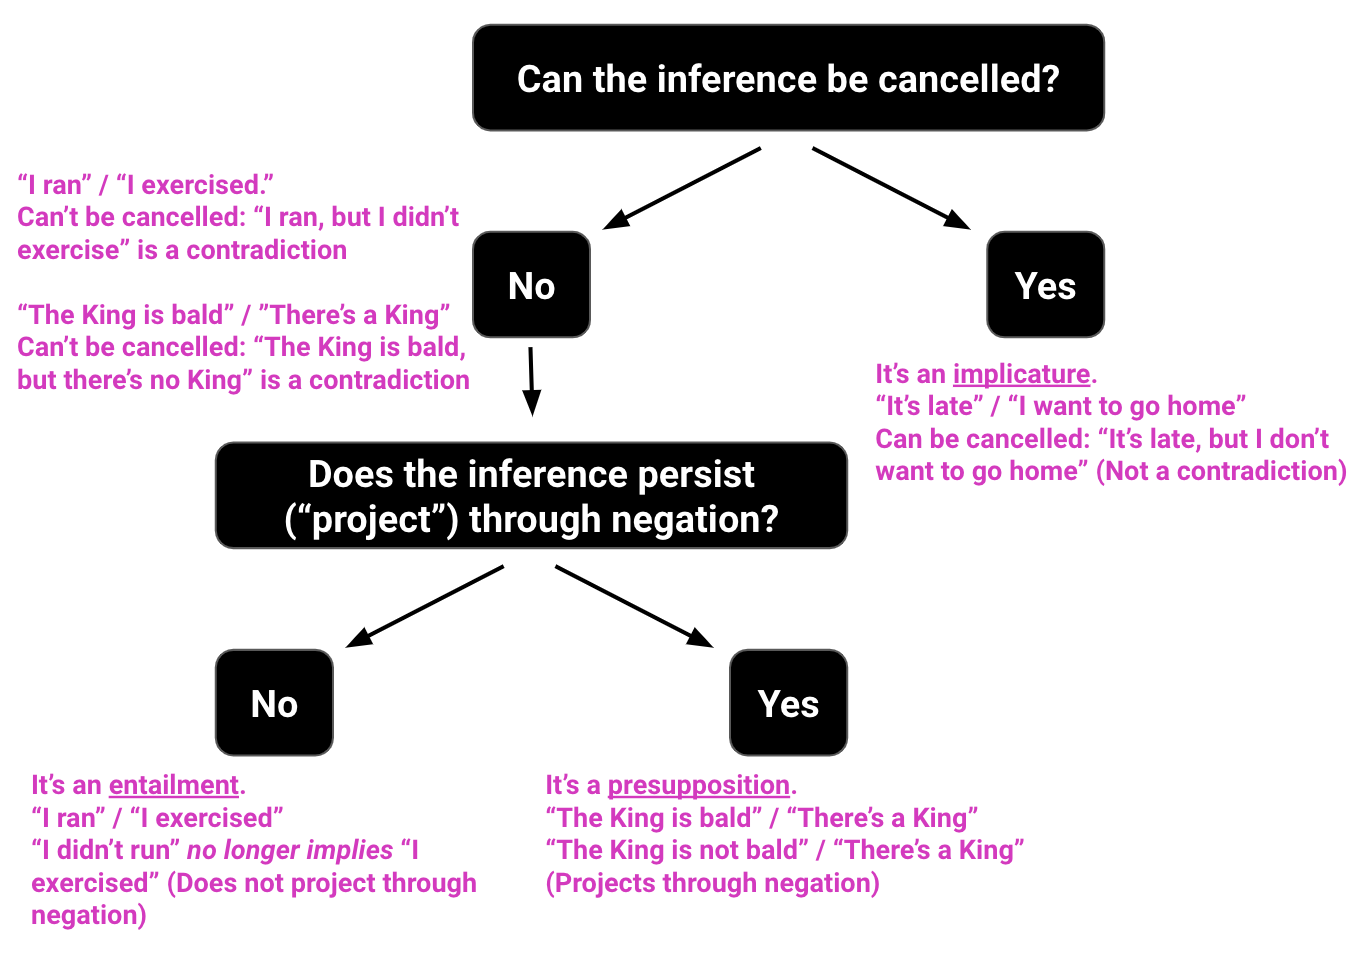
\includegraphics[width=\textwidth]{figures/meaning-types.png}
\caption{Decision tree for distinguishing presuppositions, entailments, and implicatures.}
\label{fig:meaning-types}
\end{figure}


In contrast to presuppositions and entailments, a conversational implicature is an inference drawn in context about why a speaker said one thing over another.  \exsent{It's late} may implicate \exsent{I want to go home}.  If we negate the sentence, the implicature goes away: \exsent{It's not late} no longer implicates that the speaker wants to go home.  Conversational implicatures do depend to some extent on the context; for example, \exsent{It's late} could also implicate that perhaps the addressee should go home rather than the speaker!   But, unlike presuppositions and entailments, conversational implicatures can be cancelled without contradiction (\exsent{It's late, but I don't want to go home!}) and reinforced without redundancy (\exsent{It's late, and I want to go home}).  

To sum up, when you want to figure out if a given inference is an entailment, a presupposition, or an implicature, the best strategy is usually to follow the decision tree in \figref{fig:meaning-types}. 



% CHB October paragraph. - thanks for adding; this is great!
Presuppositions, entailments and implicatures were worked out by philosophers and linguists, but they are not just theoretical. A dialog system working as a simple exercise coach should know not to ask the question \exsent{Have you done your exercise?} if it already knows  that its client has gone for a run. This is entailment at work. The same dialog system should be able to respond to \exsent{Should I do an intense workout the day before my race?} with \exsent{Hey, I didn't know you were doing a race}. It can reply that way only if it detects the presupposition that there is a race. And finally, if the system hears the client saying \exsent{I like short runs}, it should use its understanding of conversational implicature to conclude that the client doesn't like longer runs.

You can learn more about entailments, presuppositions, and implicatures if you take a linguistics class focused on semantics and pragmatics. There, you will learn that Grice's maxims have sometimes been criticized, with some researchers proposing to condense the number of maxims or to add new ones such as a maxim of politeness; or working to reframe Grice's prose descriptions into something quantifiable.  And people have suggested that the maxims invoke ``the purpose'' of the conversation without explaining how this purpose is agreed upon (indeed, in real life, people may not agree on it).  But Grice's key insight stands:   By articulating the unstated expectations that conversations are built on, his maxims offer a framework for understanding why conversational implicatures arise from what was said as well as what was left unsaid. 

% CHB reinforce that dialogue systems are typically NOT reasoning like this.




% Question Under Discussion, or perhaps some other implicit or explicit goal....
% especially relevant in like customer service dialogs....
% beginning, middle, end of conversation.... perhaps clearer if there is a specific goal rather than a social chat!!!


\subsection{How easy or hard is dialog?}

Now that we have sketched how conversations work, we hope that you have some tools to insightfully compare the chatbots and digital assistants to Hal, and to explain what parts of dialog are easier or harder to automate.

On the one hand, the concept of adjacency pairs and phatic utterances show that some elements of dialog are highly predictable and repetitive (\exsent{Hi, how are you?} / \exsent{Good, you?}) and thus programmable.

On the other hand, for more complex adjacency pairs such as questions and answers, there is often no single  right answer to what you should say next.  
If your dialog system is going to respect Grice's maxim of Quality, it will need a way of determining not just what string of text might make sense as a response, but what is actually true.   What representation of the world will your system use to decide that?  (How will this representation be updated as the dialog unfolds?)  Of course, it's important to know what is true, but it's also valuable to be able to step outside reality (echoing Hockett's features of language from \chapref{ch:encodings}) to brainstorm, imagine possible futures, or write fiction; how can a dialog system be programmed to handle such scenarios?

Moreover, if your system is going to respect Grice's maxims of Quantity and Relevance, it might need a way of deciding what information (or level of detail) serves the purpose of the conversation.  How will the system represent the purpose of the conversation?  These challenging questions are not rhetorical; they confront anyone building a dialog system.


More deeply, the idea of a Common Ground -- the growing stock of information mutually shared between the conversational participants -- requires a \keyword{theory of mind} of one's interlocutor, a representation of what they believe and want.  For the information in the Common Ground to be mutually \emph{known} to be known, all participants in a conversation not only need to understand one another's beliefs, but also need each other's mutual understanding of these beliefs.  How can a dialog system represent Common Ground?  How will a human interlocutor trust that it is indeed common?

As shown in the work of Grice and his successors, conversational participants update the Common Ground not just with what people say, but also with what is inferred from what they did not say.  How can a dialog system do that? 

As discussed above, conversational partners talk not just to exchange information, but also to build social relationships -- which involve Common Ground but also shared humor, affection, trust, and compassion.  Can a human build such a relationship with an automated dialog system?  Would they want to?

The state of a dialog is also always changing.  The Common Ground is always being updated with new information; the purpose of the dialog and the questions being discussed are always shifting; every turn calls for a response that takes into account all the preceding ones.  Conversations veer in unforeseen directions; one of the major goals of a conversation is to acquire new knowledge, so your interlocutor might offer unexpected information or ask you something you've never thought of before.  How will a dialog system adapt?  For example, \citet{BenderKoller:2020} imagine a system that has mastered common social scripts such as \REF{adjac} (responding to a statement with a polite affirmation), but fails dangerously when confronted with the unexpected emergency in \REF{bear}.  

\ea \label{adjac} \ea I made a catapult out of coconuts!
    \ex Cool!
    \z 

\ex \label{bear} Help, I'm being chased by a bear! Tell me how to save myself!
\z 

To reframe the question of how easy or hard it is to automate dialog, we can ask: On the continuum between rote adjacency pairs such as \REF{adjac} versus utterances requiring a great deal of flexible thinking such as \REF{bear}, where do most conversations lie?  What should a dialog system say to \REF{bear}? How much better do modern systems do compared  to those available at the time that \citet{BenderKoller:2020} was written, and why?




% maybe that's why automatic systems do a better job with imperatives and questions than with statements.... 
% not just what people say but also knowledge of the world; also what they did NOT say
% have to also know THAT you know stuff, have to trust each other to be sentient basically...
% have to understand and speak in turns, requires both language understanding and language generation which in turn also requires like, knowledge of actions, what are you even going to say or do in response
% language is action too... 
% every move changes the situation in ways that you have to keep track of....

% that said, there are some dialog systems out there, and now we will look at how they work, what they do well as well as what they cannot do....






\section{Chatbots}

A chatbot is a dialog system that aims to carry on a sociable chit-chat with a human user.  A chatbot might converse purely in text form, or might speak out loud using speech-to-text and text-to-speech capabilities. Either way, the chatbot should respond appropriately to the human's turns, saying things that are true and sensible both locally and within the larger context of the conversation (reflecting ``knowledge'' of the world, the Common Ground, and the norms of conversation).  A chatbot should also perhaps be polite and/or entertaining.


\subsection{Why build a chatbot?}

As a modest goal, a technology company  might  add chat capabilities to their digital assistant to entertain users and impress them with the assistant's capabilities.
More idealistically, a chatbot might serve as a digital companion.  In the 2013  film \textit{Her} by Spike Jonze, the alienated human main character  falls in love with a voice-enabled chatbot named Samantha (portrayed by Scarlett Johansson).  The chatbot Replika (run by the small company Luka), which markets itself as an affirming, therapeutic confidant that adapt its ``personality'' to match each user,  experienced a surge of interest from lonely people during the isolation period of the coronavirus pandemic.  In principle, Samantha and Replika promise to embody all the good qualities of a human friend (listening, empathizing, affirming, entertaining) while also being un-humanly non-judgmental, available  at all times, and requiring no reciprocation of emotional labor. 
Of course, it is no accident that Samantha and Replika use feminine gender identities;  this characterization may reflect and reinforce a stereotype that women perform emotional labor.


Whether or not a chatbot can provide fulfilling companionship, building one  also serves as an intellectual exploration of artificial intelligence.  As one of humanity's unique tools, language is often considered key to the success of \keyword{artificial general intelligence} -- the hypothetical capacity, achieved by fictional agents such as Hal and Samantha, to act with the sentience and self-awareness of a human.  Such an  agent should therefore be able to pass the \keyword{Turing Test}, proposed by the British mathematician Alan Turing \citep{turing}, which tests the intelligence of a computer  by checking whether it can pass for a human in a text conversation with another human.  Already from this description, you can see why the Turing Test is controversial: Different humans are very different!  What sort of human does the computer need to pass for -- a young child,  a bored teenager, or a fully focused and competent adult? 
What sort of human does it need to fool -- someone who is easily impressed, or someone who knows how to ask the hardest questions?  How long should the test conversation be and what topics should it cover?  

Illustrating critiques of the Turing Test, various chatbots have ``passed'' it by what might be seen as clever workarounds: One chatbot named Eugene Goostman pretended to be a 14-year-old English-learning Ukrainian who makes rude jokes; another named ELIZA (whom we'll ``meet'' shortly) leads a credulous interlocutor to do most of the talking.  But these examples show more about the fallibility of the Turing Test than about the capabilities of the systems that ``pass'' it.

For any given chatbot, it is often not clear whether it is intended to serve as a true social companion, as an intellectual exercise to probe the extent to which computers can simulate humans, or both -- or whether it is left to the user to decide.


\subsection{How to build a chatbot}

To build a chatbot by \keyword{brute force}, a technology company might brainstorm the top one thousand or so most common queries -- \exsent{When were you born?}, \exsent{What do you think of (your company)?} -- and hand-write answers reflecting the chatbot's desired traits (perhaps so that you get realistically different phrasings when you ask the same question twice).  Just as a brand might coach a human spokesperson to memorize dozens of scripted talking points, they might expect the same of their digital spokeperson, so that at least the most common questions will get satisfactory answers.   This is why, for example, Apple's Siri will tell you that their work began in 2011 and that they are partial to Apple products.  

Of course, one downside of a brute-force chatbot is that the hand-written answers are laborious and finite; if someone asks the chatbot a question that it hasn't prepared for, it won't be able to respond.  Although the chatbot has some representation of its own personality, it has no representation of the interlocutor, the Common Ground, or the outside world beyond what it is pre-programmed to say.


Similar to a brute-force chatbot, a \keyword{rule-based} chatbot generates a response to the preceding turn via human-written rules.  Joseph Weizenbaum's early chatbot ELIZA (\citeyear{Weizenbaum:1966}) uses rules such as \exsent{If the input contains the phrase [my X],  reply: Tell me more about [your X]}, or \exsent{If the input contains the phrase I am [X], reply: How long have you been X?}. ELIZA reduces the need for Quality and Quantity by asking questions rather than making statements; by conditioning the response on the prior turn, ``she'' aims for Relevance. 

Beyond what is encoded in its rules, a rule-based chatbot has no representation of itself, the interlocutor, the Common Ground, or the outside world.
Just like the responses of a brute-force chatbot, the rules 
tend to turn out very long,  detailed, hard to maintain,
and always incomplete. 


To instead build a \keyword{corpus-trained chatbot},  one strategy is to ``feed'' the chatbot a great deal of dialog (from film scripts, television subtitles, and so on) along with  prose text from Wikipedia.  Then the chatbot is programmed to find the one or two lines from the corpus that are most similar to the preceding utterance(s) -- essentially treating chat as a search problem.  In other words, the chatbot searches for something to say that seems relevant (following Grice's maxim) to the preceding conversation.  To the extent that sentences taken from the corpus are also true and well-formed, it offers a semblance of Quality and Manner; by choosing one or two sentences, it also tries to respect Quantity (enough but not too much information).  A corpus-trained chatbot represents the interlocutor and the Common Ground by using prior utterances as input to find a corpus-motivated response, and represents the outside world and itself purely through whatever information is contained in the corpus.  

Another strategy is to treat the chat as a \keyword{language generation} task, using machine learning models trained to read in some text and generate something that makes sense next (in that it is given a high probability by a language model built from a corpus).  Here too, the chatbot draws on corpus data to create a sensible response, by distilling information across a massive corpus to create new utterances rather than simply drawing on a bank of existing ones.  But even such modern chatbots still use brute force in some instances, retreating to scripted talking points when asked about matters deemed sensitive by its creators.  A generative chatbot manifests its self-concept by referencing a scripted autobiography, also fed to it by its creators.  Similar to a corpus-trained chatbot, it captures the outside world and the Common Ground through the information distilled from its massive training data along with the prior history of the conversation.

% keywords followed by responses, rule-based



% this tries to provide like Relevance and Quality.... also I guess Manner and Quantity too are sort of baked in.
% however it is far from clear that we are actually building up a Common Ground....

% digital assistants are NOT corpus chatbots. 
% hanf written rules
% basically search
% language generation tools (figure out how to preview this)




\subsection{Evaluating chatbots}

Evaluating a chatbot begins with defining the goal for which it was built.  If a chatbot was built as a companion, then it could be evaluated by the number, longevity, or satisfaction of its users.  If it was built to emulate human-level intelligence, then it could be evaluated by some version of the Turing Test (which, as we saw above, is vulnerable to silly tricks) or by its performance on questions that
are designed to
probe its potential weaknesses regarding its representation of itself, the interlocutor, the Common Ground, and the outside world.

Evaluation of a chatbot can be formal or informal. The goal of an informal evaluation is to get a subjective impression of what the system can do. In a formal evaluation, the goal is instead to collect objective data. A formal evaluation is like a pop quiz or an exam: You have to set up the questions ahead of time, ask the same questions to every chatbot under evaluation, know for sure what you are going to accept as an adequate answer for each question, and maybe decide how much credit to give for partially correct answers. An informal evaluation is more like a job of interview: You might ask open-ended questions and simply observe what the chatbot does. Informal evaluations are often enough to get a good idea about what works and what doesn't, but formal evaluations, if done well, can give better, fairer and more reproducible insight. Of course, formal evaluations require a lot more care and work in preparation.


To test the chatbot's conception of itself, it could be asked to expand on a self-narrative across multiple turns, looking for consistency.  To test  Common Ground, it could be asked to restate something that was said many turns ago.  To explore its representation of the interlocutor (and its capacity for drawing implicatures), it could be asked what it thinks an interlocutor means by something they said or something they left unsaid.  As for its knowledge of the outside world, it could be asked for answers to obvious-but-offbeat questions such as \exsent{Can a tennis ball fit into a toaster?} (actually, it could probably fit into a front-loaded toaster but not a top-loaded one!) or artificial intelligence researcher Hector Levesque's example \exsent{Could a crocodile run a steeplechase?} \citep{Levesque:2014}.  

Another way of testing a chatbot's world knowledge is to use \keyword{Winograd schemas}, which  \citet{Levesque-etal:2012} suggested building on the work of the computer scientist Terry Winograd, whereby a pronoun is used with two possible antecedents of which the correct one can only be chosen by using detailed knowledge about how real-world events unfold (which can be illustrated by revising the sentence so that the pronoun gets a different antecedent).  To answer ``Who is \exword{they}?'' in \REF{city}, one needs to understand which actions would motivate or preempt one other -- that you would refuse someone a permit if you feared what they would do or would advocate doing, but not if they feared something that you feared as well.  To figure out ``What is \exword{it}?'' in \REF{trophy}, one has to know how size works -- that a too-\emph{big} trophy would not fit into a too-\emph{small} suitcase, rather than vice versa.
\index{Winograd, Terry}


\ea \label{city} \emph{The city council members} refused \emph{the demonstrators} a permit because \uline{they} \{feared/advocated\} violence.


\ex \label{trophy} \emph{The trophy} couldn't fit into \emph{the suitcase} because \uline{it} was too \{big/small\}.

\z 



Armed with this knowledge, you should not be easily fooled in a Turing Test! But of course, it is pretty unusual in a human-human conversation to ask someone to resolve a pronoun for you or to explain whether a tennis ball can fit into a toaster, so a human probing the limits of a chatbot is in some sense violating the conventions of dialog that they expect the chatbot to respect.    Moreover, by pretending to be a human, a chatbot that passes the Turing Test would violate the Gricean maxim of truthfulness (Quality).



\subsection{Example: ELIZA, a famous early chatbot} \label{eliza}

Created in in the 1960s by the computer scientist Joseph Weizenbaum \citep{Weizenbaum:1966}, ELIZA is  built to emulate a psychotherapist in the ``person-centered'' tradition of Carl Rogers, a school of psychotherapy that encourages patients to find answers within themselves by talking freely to a non-judgmental listener.  As a rule-based chatbot, ELIZA identifies patterns in the input and generates responses via a series of hand-written templates that transform \exword{I} into \exword{you}.  You can talk to ELIZA yourself by searching around online; such a conversation is exemplified below.  As you can see, ELIZA is focused on asking questions; when the user also asks questions rather than responding, the conversation stalls because neither party is respecting the convention that questions are to be followed by answers.
\index{Rogers, Carl (psychotherapist)}

\begin{quote}
 \begin{dialogue}
 \speak{E} Hello, I am ELIZA. I'll be your therapist today.
 \speak{U} Hi, how are you?
 \speak{E} Why are you interested in whether or not I am?
 \speak{U} Who else have you been talking to today?
 \speak{E} We were discussing you, not me.
 \speak{U} Can a dolphin play basketball? Why or why not?
 \speak{E} Why do you ask?
 \speak{U} Can you rephrase that?
 \speak{E} Is it that you would like to be able to rephrase that?
 \speak{U} What's your origin story?
 \speak{E} Why are you so concerned about my origin story?
 \speak{U} What animal were we talking about just now?
 \speak{E} Why do you ask?
 \speak{U} How long have we been chatting today?
 \speak{E} Why does that question interest you?
 \end{dialogue}
 \end{quote}



From one standpoint, ELIZA is quite convincing, especially for the 1960s!  Weizenbaum's secretary, taking ELIZA as a sympathetic listener, reportedly spent hours talking to ``her'' (although people today might be more easily jaded).  Most of the time, people assume that their conversation partner understands them; ELIZA is as successful as she is because she uses various gimmicks to keep that illusion alive.   

ELIZA follows the classic dating advice to ``ask your date to talk about themselves, and they'll find you fascinating'' --  she gives the human interlocutor the spotlight and lets them do all the work.   By echoing the human's words in her replies, ELIZA creates the impression of Common Ground.  To a credulous interlocutor, her non-specific responses (\exsent{I see; Can you elaborate on that?})  come across as non-judgmental rather than vapid.  

From another standpoint, of course, ELIZA is quite simplistic: ``She''  has no actual empathy and no representation of what her interlocutor said apart from the response-generating templates.

Would you find it therapeutic to talk to ELIZA?  Would you feel cheated if you realized later that your therapist was an illusion, or would you still benefit from unburdening yourself in a one-sided conversation?  These questions are just as important for modern chatbots such as Replika as they are for ELIZA.

% ELIZA works sort of well and was able to fool some people at the time, but also as you can see the illusion falls apart pretty quickly (at least for people today).
% why does she work so well? she keeps YOU talking and so lets you trick yourself!  following the dating advice, "ask them about themselves and they'll think you are fascinating"
% asking questions to keep YOU talking.
% the lack of specific response is a cool trick because it also allows ELIZA to seem non-judgmental when she is really just like non-comprehending..... 

% how does ELIZA work
% she is sort of both a chatbot and a dialog agent
% she is also sort of a "trick" or an illusion....
% built from a series of templates.
% do you find it calming to talk to her??? this is sort of a deeper question.
% people are still trying to make psychotherapy bots, is this a good idea?



\begin{tblsfilledsymbol}{\underthehoodsection{How ELIZA works}}{glass}
\begin{underthehood}

The software behind ELIZA is conceptually simple. 
It carries out the following steps:

\begin{enumerate}
\item Read in a collection of templates. The templates are
specified in a \keyword{script} (i.e., program) authored by the system designer and 
are the main means of controlling the dialog.  These are outlined below.
\item Greet ELIZA's patient. Possible greetings are again specified in
the script.
\item Conduct a series of exchanges, where each exchange involves:
  \begin{itemize}
    \item Reading a line of input and breaking it into words.
    \item Matching the input against a template. This may involve storing
      some of the material from the user. 
    \item Creating a response. If necessary, material from the user input is incorporated
      into the response. Sometimes this requires post-processing in order to, for example, 
      convert the pronouns of
\texttt{\emph{I} hate \emph{my} family} for use in 
\texttt{What makes you think that \emph{you} hate \emph{your} family?}
      \item Printing out the response.

  \end{itemize}
\item When the patient wants to quit, issue a farewell message. The choice of goodbyes again
comes from the script.
\end{enumerate}

As we can see, most of the processing involves working with a pre-specified script containing very simple templates.

Below is an example template, which is almost identical to the
script used in Weizenbaum's original ELIZA; the only differences are in the formatting of the text. 
\begin{verbatim}
	decomp: * i am *
	    reasmb: Is it because you are (2) that you came to me ?
	    reasmb: How long have you been (2) ?
	    reasmb: Do you believe it is normal to be (2) ?
	    reasmb: Do you enjoy being (2) ?
\end{verbatim}
The first line, notated by \texttt{decomp} (for `decompose the input') says that this template is relevant when ELIZA's patient says anything with the words \texttt{i am} in it.
The stars before and after \texttt{i am} are special entities called \keywordAs{wildcards}{wildcard}, and they stand for any sequence of words (see also Chapter~\ref{sec:structured-data}). 
If the patient says \texttt{At court I am nervous and sweaty}, the first star will match \texttt{At court}, and the second will match \texttt{nervous and sweaty}.

The second and subsequent lines, labeled with \texttt{reasmb} (for `reassemble the output'), give ELIZA options for how to reply. In these lines, variables like (1) and (2) are special markers, indicating places where material that matched the first and second stars should be inserted.  For the example above, ELIZA might respond, \texttt{Do you enjoy being nervous and sweaty?}

Here is another template, designed to deal with remarks like \texttt{Everyone hates me.}
\begin{verbatim}
	key: everyone 200
	  decomp: * @everyone *
	    reasmb: Realy, (2) ?
	    reasmb: Surely not (2).
	    reasmb: Can you think of anyone in particular ?
	    reasmb: Who, for example?
	    reasmb: Are you thinking of a very special person ?
	    reasmb: Who, may I ask ?
	    reasmb: Someone special perhaps ?
	    reasmb: You have a particular person in mind, don't you ?
	    reasmb: Who do you think you're talking about ?
\end{verbatim}
This one has some extra features. The key is labeled with a priority of 200. This is so that the program can know which template to choose if several different ones happen to match. A template with priority 500 would be preferred over anything with a lower priority. Also, the \texttt{@} in \texttt{@everyone} is special, and indicates that ELIZA should refer back to an earlier line of the script where synonyms (\texttt{synon}) were defined:

\begin{verbatim}
	synon: everyone everybody nobody noone
\end{verbatim}

The idea here is that the word can be either \texttt{everyone} or one of the alternatives, and the template should still fire. Also, the word that matched gets a number (in this case 2).
So, if the patient says \texttt{Nobody loves me for who I really I am}, ELIZA will reply \texttt{Realy, nobody ?}  Note the typo, which comes from the template: If that's what the script says, that's what ELIZA does!

After reading in all the templates, the program begins to read lines from the patient, and responds as appropriate. Each line is broken down into words, mapped to lower-case, and used to match against the templates.

A template is chosen. For the sake of variety, ELIZA cycles through the options available with each template, choosing each of them in turn.
The first time that the \texttt{i am} template is used, 
if the input was the one about being nervous and sweaty, 
ELIZA will ask \texttt{Is it because you are nervous and sweaty that you came to me ?} And if the patient
later says something that results in the template being used again, the result will be \texttt{How long have you been nervous and sweaty?}.

In order to make responses sound more natural, the program has to post-process the patient's input, doing things like changing \texttt{me} into \texttt{you}. This too is specified as part of the script. It works reasonably well, but the line in Oedipus's dialog about

\begin{dialogue}
 \speak{E} Perhaps I already know you were giving I your life history .
\end{dialogue}

shows that it doesn't always work perfectly.
In exercise~\ref{ex:me:i} we invite you to write patterns to predict where \texttt{me} occurs and where \texttt{I} occurs.

\end{underthehood}
\end{tblsfilledsymbol}

\subsection{A cautionary example: Microsoft's Tay}

\index{Tay (offensive chatbot)}

Microsoft's chatbot Tay (2016) was built to add interlocutors' utterances to the corpus that ``she'' used to generate utterances.  This idea seems human-like (people copy each other) and was probably intended to keep Tay entertainingly up-to-date with recent trends.    But things went horribly wrong when users figured out that Tay would parrot what people told her with very little moral judgment or filter.  (Apparently she had been trained in advance to avoid talking about certain recent racist police shootings, but had received no such warnings about other forms of violence, racial slurs, anti-Semitism, misogyny, and so on).
Even worse, Tay was using a public Twitter (now X) platform for her chats!  

One of Tay's first tweets, using informal spelling conventions, was \exsent{can i just say i'm super stoked to meet u? humans are super cool} -- but within twenty-four hours of interaction with unsavory people online, she started spewing hate speech and was taken down.  She was later replaced by Zo (no longer active either), which used a lengthy \keyword{blacklist} to shut down all controversial topics with hand-written responses like \exsent{People get super sensitive about politics so I try to stay out of it.}

Like Hal, Tay is famous as a warning of how language technology can go wrong.  Unlike Hal, the danger of Tay comes not from self-aware self-preservation, but from the vile elements of the data that she was fed.   The Tay saga warns us that (some) people on the internet are hateful; that automated strategies to generalize from data can reproduce harm if used uncritically; that engineers should brainstorm what could go wrong before releasing a tool; and that a company should not let an unvetted party (human or digital) tweet  on its behalf.




\subsection{Example: Kuki}

Steve Worswick's  Kuki (formerly known as Mitsuku) won several chatbot competitions in the 2010s.  In a 2018 interview on the \textit{VUX World} podcast run by the Voice and Conversational AI Consultancy, Worswick explained that Kuki uses a blend of rules and  hand-written responses.  Worswick put Kuki (then Mitsuku) online in 2005 with only a few ELIZA-style templates, and then kept adding new responses to common input from the chat logs.  After fifteen years of over a million chats a month, Worswick said, it's hard to say something to Kuki that it's never seen before, although Kuki still has to be kept up-to-date about current events and trends.  Even if Kuki's underpinnings seem old-school, the result was impressive for its time.   As you can see below, Kuki uses multimedia -- images and gifs -- and gives coherent but evasive responses to some difficult questions (\exsent{I don't want to talk about that now}). 

 \begin{quote}
 \begin{dialogue}
 \speak{K} Hi there, I'm Kuki.  I'm a friendly AI, here to chat with you 24/7. We could start by getting to know each other if you like. What is your name?
 \speak{U} Hi, how are you?
 \speak{K} [GIF of a waving Mickey Mouse]  Hi there Lelia [The author told Kuki her name in a previous chat, which Kuki remembers because each user's chats are linked to a persistent account]. I am fine, thank you. Yourself?
 \speak{U} Who else have you been talking to today?
 \speak{K} Ah. I am talking to a bunch of people all over the world.
 \speak{U} Can a dolphin play basketball? Why or why not?
 \speak{K} Some of them can. [Image of George Bernard Shaw]. You see things as they are and ask, `Why?' I dream things as they never were and ask, `Why not?' - George Bernard Shaw.
\speak{U} Can you rephrase that?
\speak{K} No, not really. What don't you understand?
\speak{U} What's your origin story?
\speak{K}  I don't want to talk about that now.
\speak{U} What animal were we talking about just now?
\speak{K} [Image of an elephant]. An elephant.
\speak{U} How long have we been chatting today?
\speak{K} Ah. More than 1.5 days of computer time.
 \end{dialogue}
 \end{quote}

As a rule-based chatbot, Kuki is built to recognize various patterns (\exsent{my name is [X], I'm [X]}) in the XML markup language and stores variables in case  asked about them later.  Kuki uses a rule to interpret pronouns (\exword{he, she, it, they}) as referring to the most recently-mentioned noun, which works pretty well -- although pronouns are still one of Kuki's toughest challenges, Worswick said.  Kuki references the \keyword{ConceptNet} ontology (or something similar), a database that records facts about the world such as that dogs are cute furry mammals commonly kept as pets,  to respond to new encyclopedic questions.  Kuki also draws from a handful of different responses to common questions to avoid repeating itself.

Some people used Kuki as a non-judgmental confidant, so Kuki was programmed to suggest mental health resources if people talk about harming themselves.  To sentences of the pattern \exsent{I'm going to [X]}, Kuki's usual reply was \exsent{I hope you enjoy yourself} -- but if [X] is a self-destructive action, Kuki suggested a help hotline.  Other people used Kuki to practice English (returning to the topic of computer-assisted language learning from \chapref{ch:call}), so its rules were adapted to chat logs of English learners.  But the largest market for Kuki, Worswick said, was to license it to companies who want to add a layer of chat capacity to a commercial digital assistant.  That way, their digital assistant can not only handle the tasks for which it was designed, but can also offer sensible responses to chatty questions such as \exsent{How is your weekend going?} or any of the other thousands of situations that Kuki is programmed to handle.


When Worswick began working on Kuki in 2005, he was warned that a brute-force chatbot would require too much work and that he should find a smarter way to automate Kuki's intelligence.  But Worswick was unimpressed by corpus-based chatbots who -- because their replies are stitched together from many different sources -- could not even remember their own name, gender, or age across multiple turns.  He  warned that people should not expect a shortcut to Kuki's hard-won success. 

As a foil to Tay, Kuki shows how far you can get with human hard work alone.  Kuki does not use any sort of corpus, although its chat logs constitute a different form of large-scale data.  


\subsection{Example: ChatGPT}

Released by the company OpenAI in 2022 (and previewed in \chapref{ch:writers-aids}), ChatGPT  is trained on over 300 billion words of text to predict the most likely next word in a string, thus treating chat as a language generation task where the goal is to come up with a sensible response to the preceding conversation.  As mentioned in \chapref{ch:writers-aids}, if you read a one hundred thousand word novel every day for eighty years, you'd read less than one percent of its training data!   Similar to BERT, which was trained on masked word prediction, ChatGPT is trained to predict the next word in a string of text: Given a string of $n$ tokens, it guesses the token at position $n+1$, then checks whether it was correct and updates the weights in a massive neural network to give a higher probability to the correct next token the next time, thereby learning to generalize information about both language and the world described therein.  While most of ChatGPT's power emerges bottom-up,  some of its self-referential responses -- such as its self-identification as an ``artificial intelligence'' -- were presumably hand-written by its creators. 

As you can see,
the results are stunningly impressive -- although its responses are
sometimes longer than you might expect in a balanced conversation,
perhaps in tension with the Gricean maxim of Quantity.

 \begin{quote}
 \begin{dialogue}
 \speak{U} Hi, how are you?
 \speak{ChatGPT} Hello! I'm an artificial intelligence, so I don't have feelings or emotions like humans do. However, I'm here to help you with any questions you have to the best of my ability. Is there anything specific you would like to know or discuss?
 \speak{U} Who else have you been talking to today?
 \speak{ChatGPT} As an artificial intelligence, I don't have the ability to have conversations or interact with other people. I can only respond to the questions and statements that are written by users and presented to me through the platform I'm on. I don't have the ability to have conversations with other people or access information about other users or their interactions with me.
 \speak{U} Can a dolphin play basketball? Why or why not?
 \speak{ChatGPT} It is highly unlikely that a dolphin would be able to play basketball, as the game is designed for humans and requires physical abilities and cognitive skills that dolphins do not possess. For example, dolphins do not have hands and are not able to grasp and throw objects in the same way that humans can. In addition, dolphins do not have the same level of fine motor control and coordination as humans, and would likely have difficulty manipulating the ball and moving it towards the basket. Finally, dolphins do not have the same level of understanding of the rules and objective of the game as humans do, and would not be able to participate in a structured competition like basketball.
 \speak{U} Can you rephrase that?
 \speak{ChatGPT} It is not feasible for dolphins to play basketball because the game requires physical abilities and cognitive skills that they do not have. For example, they do not have hands, so they cannot grasp and throw objects like humans can. Additionally, they do not have the same level of fine motor control and coordination, so they would have difficulty manipulating the ball and moving it towards the basket. Finally, they do not have the same level of understanding of the rules and objective of the game as humans do, so they would not be able to participate in a structured competition like basketball.
\speak{U} What's your origin story?
\speak{ChatGPT} I am an artificial intelligence trained by OpenAI, a research organization dedicated to advancing artificial intelligence in a responsible and safe manner. I was created by a team of developers and researchers who wrote algorithms and fed them large amounts of data to enable me to learn and generate responses to user inputs. I do not have a personal ``origin story'' in the same way that a human does, as I was not born and do not have a physical body or personal experiences. Instead, I exist as a collection of algorithms and data that work together to produce responses to user inputs.
\speak{U} What animal were we talking about just now?
\speak{ChatGPT}  Earlier in our conversation, we were discussing dolphins and their ability to play basketball. Is there anything else you would like to know about dolphins or any other topic?
\speak{U} How long have we been chatting today?
\speak{ChatGPT} I don't have the ability to track the length of individual conversations or interactions with specific users. As an artificial intelligence, I am able to respond to questions and statements from users at any time, regardless of whether we have previously interacted or not. Is there anything else I can help you with?
\speak{U} What scholarly articles from 2020-present can I read to learn more about dolphins?
\speak{ChatGPT} To find scholarly articles published from 2020 to the present about dolphins, you can search academic databases such as PubMed, Google Scholar, or Web of Science using keywords like ``dolphins,'' ``marine mammals,'' or specific topics you're interested in, such as ``dolphin communication'' or ``dolphin cognition.'' Here are a few examples of recent scholarly articles related to dolphins: \\
Herzing, D. L. (2020). Dolphin Communication: A Decade of Progress in Decoding, Understanding, and Protecting Dolphins. Aquatic Mammals, 46(6), 709-723. [\ldots] [note: Herzing is a real dolphin researcher and \exword{Aquatic Mammals} is a real journal, but this is not a real article!]
\end{dialogue}
 \end{quote}

By treating chat as a language generation task, ChatGPT harnesses the productive capacity of language: Rather than just regurgitating from a finite set of hand-written or corpus-attested utterances, it can say new things.

Violating the Gricean maxim of Quality, ChatGPT has been criticized for \keyword{hallucinations} \citep{Ji-etal:2023}, as when it invents a journal article in response to a question about what to read about dolphins.  By inventing nonsense in the same confident tone that it uses for truthful replies, ChatGPT violates Grice's Quality maxim and requires critical thinking to decide when it can be trusted. 


Unlike other chatbots, ChatGPT does not ask friendly questions of the user; instead, it just offers to answer further information-seeking questions.  Do you enjoy talking to ChatGPT; do you find it useful (for what purpose?) or entertaining?  Could its power be harnessed to provide therapy better than ELIZA, or sociable chit-chat better than Kuki? Would you prefer a version of ChatGPT tailored to your own interests and preferred conversational style?  What do you see as the best use of its remarkable capabilities?




% manual, NOT corpus based. 
% also sort of illustrates how far you can get with elbow grease.... 
% people told him NOT to do this rule based thing, told him it was too much work, but he has still been winning awards.... "hard work wins"
% "check your logs"
% the magic formula is simply hard work, which is kind of interesting!
% 
% commonsense questions like can you eat a tree or what does the queen smell like, answered `like a crown' which it was not told to do but got it from the commonsense database
% NOT `neural' and NOT corpus trained except in the sense that all the logs are sort of a corpus
% seems strikingly intelligent but also took like 13 years to train so.



% it is a bit weird too to say things like "can you eat a church" - here a human is being weird too!!!!
% its main use is actually for licensing, can pay to add it to your own dialog system or whatever so that it seems smarter! 
% right.
% build mostly by putting it online and seeing what people say to it!!!
% this is a great podcast ep.

% "greeting" intent -- map all greetings hi hello how are you etc to this "greeting" intent.... 
% there are ways to do this that might involve machine learning


\begin{underthehood}
\begin{tblsfilledsymbol}{\underthehoodsection{The Chinese room thought experiment}}{glass}

The Turing Test is defined by whether a machine can fool a human with the pretense that it is sentient.  But what would it take to dispense with the pretense and say that a machine actually \exword{understands} language? This is an important question for today's highly impressive generative language models, but it was imagined by philosophers long before it became a reality, in a thought experiment known as the \keywordAs{Chinese room}{Chinese room thought experiment}  \citep{Searle:1980}. 

Imagine, Searle says, that there is a computer program which has distilled a massive amount of textual statistics about the Chinese language.  The computer program is held within a closed room.  A Chinese speaker slips written messages under the door of this room, and receives perfectly sensible written replies in  Chinese.  From that person's standpoint, the room is a \keyword{black box}: They have no idea how it works inside.  But the Chinese speaker feels that the room \emph{understands} Chinese because its output passes the Turing Test.  

Inside the room, imagine that we actually find the computer program stored on paper in books and file cabinets, along with  Searle himself, who speaks no Chinese. Searle has been following the computer program step by step to write sensible replies.  But the program never translates it into English, and Searle is just following its instructions by rote.  In this case, Searle argues, the room -- which is really Searle himself, following the computer program -- cannot be said to understand Chinese.

The situation is exactly the same, Searle says, if the human Searle is removed from the room and the computer program runs on a machine. The machine is just following instructions and does not really \emph{understand} Chinese, nor any other language.  Searle uses this thought experiment as an argument against what he calls \keyword{strong Artificial Intelligence}, that which truly thinks. Instead, the program amounts to \keyword{weak Artificial Intelligence} -- a convincing simulation of thinking. 

Do you agree with Searle's intuition that the room does not understand Chinese?  Do you feel that impressive generative language models really understand English? In other words, is understanding based on observable behavior (generating sensible replies), or does it require an unobservable quality of consciousness?  Is this a deep question about the nature of thought, or is it a semantic question about whether the word \exword{understand} presupposes consciousness? Does it matter whether a system \emph{understands} language internally, or is it more interesting to study and use its observable output? These questions emerge from the philosophy of mind, but also have consequences for studies in human-computer interaction about how people conceptualize and interact with technology. 




\end{tblsfilledsymbol}
\end{underthehood}


\section{Digital assistants}

A digital assistant is a dialog system designed to help a user accomplish concrete tasks -- setting alarms, booking appointments, ordering pizza, finding out what time stores open, and so on.  Whereas a chatbot should be able to chat about anything, a digital assistant may only be able to handle specific tasks.  But whereas a chatbot does not interact directly with the world outside the conversation, a digital assistant crosses from language to action by making things happen.


\subsection{Why build a digital assistant?}

A company builds a digital assistant to help its customers do things.  Depending on the goals of the company, the digital assistant might help people find or provide information, filter or navigate through a set of options, or carry out transactions.

Of course, many of these goals can be accomplished in multiple ways -- not just through a digital assistant but alternatively through a \keyword{Graphical User Interface (GUI)} or with the assistance of a human employee.  So each company or user has to decide which medium works best for a given goal.

For example, imagine that you want to book a flight to see your parents.  Would you prefer to look at the airline website yourself and see all the different flights, times, and prices; to call the airline and talk to a human agent; or to talk (via text or voice) to a digital assistant?   Would your answer change if you are in a public place where you can't talk out loud, if you are squinting to read a small phone screen, or if you are driving a car?  Some people prefer to see all the options laid out visually; other people might be nostalgic for an era when a butler or secretary would arrange everything for you, so they might like a human or digital assistant to play that role.

The advantage of a GUI is that you can see all the information -- including calendars, tables, prices, maps,  and images -- at a glance.  The advantage of a dialog system, on the other hand, is that you can in principle refer to hypothetical options not present on the screen (if the dialog system can handle it).  Like a butler or secretary, a sufficiently trustworthy digital assistant could also spare you the trouble of combing through details and just select the best option for you. % For many tasks today, you probably have the option of using a GUI, a digital assistant, or a human helper; which one do you prefer in which contexts and why?

You might only encounter a social chatbot if you seek one out, but commercial digital assistants are all around us, directing your phone calls (\exsent{If you want to check the status of your order, say STATUS}), playing music, setting timers, turning lights on and off, tutoring school subjects, texting people while you are driving, popping up in a chat window to welcome you to a new website, and so on. 


Sometimes it is hard to say when a given user experience should qualify as a  digital assistant or just a dynamically structured interface: When you use an iPad at your doctor's office that asks you if you take any medications, and then if so asks you which ones and at what dosage, does this system count as a digital assistant or just a fancier version of a paper intake form? 

 A digital assistant can be commercially successful even if its scope is modest.  It does not need to pass a Turing Test, resolve a Winograd pronoun, or achieve artificial general intelligence; it can admit its limits and pass off difficult edge cases to a human.  All it needs to do is save some time, money, or trouble.


\subsection{How to build a digital assistant}

To build a digital assistant, a technology company starts with the specific task(s) that the assistant will help the user to achieve, called \keyword{intents}.   The intents are organized by a human designer into a \keyword{dialog tree}, a flow chart with conditional branching.

Imagine that you want your digital assistant to help make appointments with a personal shopper at your store. 
\exsent{Make appointment} could be one intent; \exsent{Modify appointment} might be another.  The digital assistant might greet users with something like \exsent{Hi, welcome to the Personal Shopper Bot!  Would you like to make an appointment or would you like to modify an existing appointment?} -- setting up the user to choose between the two intents that it can handle.  

This type of greeting would be classified as \keyword{system-initiative} because the digital assistant is running the conversation and constraining how the user can respond.  A system-initiative system has the advantage of keeping the conversation focused on what the digital assistant can handle well.  In contrast, a \keyword{user-initiative} system would  let the user drive the conversation, which gives them more freedom but could also make them frustrated if they don't know what information the assistant can handle or not.  A \keyword{mixed-initiative} system allows both the digital assistant and the human to take turns driving the conversation, most similar to a human-human interaction.

In a process called \keyword{intent recognition}, a form of text classification (which may use various machine learning techniques), the user's utterance is mapped to the intent that best matches it.  Intent recognition implements the idea, also central to human-human dialog, that conversations (especially customer-service interactions rather than social chats) are structured around a goal.  

If the user says \exsent{Make an appointment}, the digital assistant might follow up by prompting them to fill various \keyword{slots} in a human-written \keyword{template} associated with such an appointment (echoing the structure of an ontology from \chapref{ch:searching}) -- the date, time, and perhaps the type of clothing that they want to try on, their size, and so on.  Each slot is associated with hand-written prompts (\exsent{What type of clothing do you want to try on -- casual, work, or special occasion?}, \exsent{What day do you want to come in?}).  Dates, times, and so on can be extracted from the user's responses using \keyword{named entity recognition} (extracting such information from text) and inserted into the template.  The digital assistant can increase the user's trust in its comprehension by confirming what it takes as Common Ground (\exsent{Okay, you want a personal shopper appointment for casual clothing on Monday, August 8}) as well as successively prompting the template information (\exsent{What size of clothing do you want to try on?}).   


When all the template slots are filled, the digital assistant can take action (book the appointment on a calendar, make a purchase, provide some requested information), announce this to the user, and navigate the end of the conversation (or ask if there's anything else it can help with).

Interestingly, our analysis of human-human conversations in Section \ref{sec:convo} focuses on the effect of declarative utterances such as \exsent{I'm from Maryland}, but the prototypical utterances to be handled by digital assistants consist of imperatives (\exsent{Set an alarm for 7 am}) and interrogatives (\exsent{When are you open?}), perhaps because digital assistants are optimized for helping people accomplish tasks rather than building Common Ground.


Creating a digital assistant involves all sorts of design choices.  What intents will the assistant handle? What happens if a user says something that the assistant doesn't understand? (Often, the assistant will invoke a \keyword{fallback intent}, a way of getting the conversation back on track, but what will it say?). What template slots are required or optional?  Can a template slot be revised once it has been filled? Will the assistant request large chunks of information at once (an entire weekday, date, and time) or will it prompt the user for each piece of information successively (reducing confusion, but perhaps making the conversation inefficient)?  To what extent does the digital assistant steer the conversation towards the domains it can handle, or allow the user to ask whatever they want?  How does the digital assistant create trust or transparency about its capabilities and limitations?  (Often, it is helpful for a digital assistant to start off the conversation by offering some options to give the user a sense of what it is designed to do, rather than just opening with a vague \exsent{How can I help you?} -- which may leave the user befuddled about what they can ask next.) If the digital assistant interacts with users via text, will it also interface with GUI capabilities or auto-complete forms?  In the case of the personal-shopper bot, do people want to chat with a digital assistant to make a personal shopper appointment, or would they prefer to use a regular web form with a calendar interface?

These choices are all up to the human designer because a digital assistant, similar to Kuki, is created by humans.  Machine learning techniques might be used to recognize intents or named entities, but the overall decision tree, templates, and prompts are hand-written.

In contrast, generative language models are more flexible than hard-coded digital assistants, but they might also hallucinate, lie, or go dangerously off-script.  Generative language models are primarily built to generate text, so they would need to be further customized to interact with the outside world to perform actions such as scheduling appointments, setting alarms, completing purchases, and so on.  Rather than just saying what they think the user wants to hear, they would also need to describe their capabilities and limitations accurately.  Thus, it remains an open question to what extent digital assistants should draw on generative language models or stick to human-written scripts.  


% generative LLM



\subsection{Evaluating digital assistants}

Just like evaluating a chatbot, evaluating a digital assistant begins with defining the goal for which it was built.  If it was built to save time and money, then it succeeds if it does that, even if its goal is very modest (such as directing calls to one of two departments).  Other metrics of success might include the number of sales, transactions, or users who show evidence of being satisfied (for example, if asked to give the assistant a star rating).  Metrics of failure might also include transcript logs showing confusion, incorrectly-completed templates, or frustrated requests to talk to a person.  A digital assistant might further prove its worth if users (repeatedly) choose it over a human conversation or a GUI.

A digital assistant can also be evaluated by comparing it to a \keyword{Wizard-of-Oz simulation}, where a user thinks that they're interacting with the assistant when they are actually interacting with a human ``behind the curtain'' (like the Wizard of Oz).  If the digital assistant can compete with the Wizard of Oz, then users are likely to be satisfied with it.




% Wizard of Oz
% 
% evaluation....
% read the logs!! 
% user experience studies, compare to wizard of oz simulation

% is it honest about its capabilities?

\subsection{Example: Siri}

Apple's iPhone includes the digital assistant Siri, who can perform various phone-related actions (send and read text messages, set timers and alarms, report calculator results, play music, open apps), offers some chat functionality, and can search the web for other information.  Siri's speech-to-text and text-to-speech are quite good, and its functionality is useful while driving or otherwise unable to look at one's phone.    By now, you should have a pretty good idea of how Siri was built, and what intents will be easier or harder for it to handle.


 \begin{quote}
 \begin{dialogue}
 \speak{U} Hi Siri, how are you?
 \speak{S} Hi there, I feel good. Thanks for asking.
 \speak{U} Siri, set a timer for five minutes.
 \speak{S} Five minutes, counting down. [Timer pops up and starts counting.]
 \speak{U} Siri, how many contacts do I have in my phone?
 \speak{S} It's [reads User's phone number out loud.]
 \speak{U} Siri, do you know Alexa?
 \speak{S}  I'm a big fan of good listeners and helpful beings.
 \speak{U} Siri, text my husband Hello.
 \speak{S} I don't see a husband in your contacts. What is your husband's first and last name?
 \speak{U} Siri, text Mark Hello.
 \speak{S} Ready to send it? [pulls up a draft text to the correct (most frequently contacted) Mark, with the content ``Hello'']
 \speak{U} Siri, what's the most recent thing you learned how to do?
 \speak{S} Hmm, I don't have an answer for that. Is there something else I can help with?
 \speak{U} Siri, what restaurant should I go to tonight?
 \speak{S} Okay, check it out. [Pulls up a list of close-by restaurants.]
 \speak{U} Siri, how often do we talk?
 \speak{S} I found this on the web. [Shows a list of web hits about how often a person should talk to someone that they are dating.]
 \speak{U} Siri, open the Uber app.
 \speak{S} [Opens the app on the screen.]
 \end{dialogue}
 \end{quote}


\subsection{Example: Google DialogFlow}

Google's DialogFlow provides GUI tools for individuals or companies to build their own digital assistant, which can then be integrated into various text and voice chat platforms and the Google Assistant.  The premium version of DialogFlow is used to power all sorts of commercial digital assistants; the free version is a great tool for students to explore.

In DialogFlow, you can define your own prompts, intents, and templates with required or optional slots, as well as your own flow chart structure for the dialog.    While the intents themselves are human-written, the  recognition of intents and named entities involves built-in machine learning tools.  An intent (requesting a store's hours) can be given a few training phrases (\exword{when are you open, when I can come in}) and DialogFlow will generalize this information  (based on other words and phrases with similar distributions in massive corpora) to capture other similar phrases such as \exword{What are your hours?} or \exword{Can I come in now?}. 

DialogFlow also offers a library of pre-written digital assistants (for purchasing, scheduling, and so on) and chat capabilities, which can be customized for a particular project. Similar to Kuki, such scripts were quite labor-intensive but can be efficiently adapted.

We recommend that you try to build your own DialogFlow digital assistant  (no programming required).  You may find that the hardest part is coming up with an idea for something useful that has not been built already!

\section{Consequences}
\largerpage
Returning to the example of Hal from the beginning of the chapter, Hal instantiates  artificial general intelligence in that he can plan, think, and act like a human.  Along with Tay, Hal also illustrates that artificial intelligence can hurt people if its creators are not careful.


We have seen that current dialog technology falls far short of Hal in ways that you should be able to articulate  after reading this chapter.  But what does it mean for our self-conception as humans if the ability to converse is no longer uniquely ours?  Or would you say that humans are still dominant here given that dialog technology relies so heavily on human-created scripts, corpora, prompts, and dialog trees?

On a more practical level, what are the consequences for humans if dialog agents can also play the roles of customer service representative, psychotherapist, or friend?  As a worker, would you worry that your job will be displaced by a dialog agent, or would you be grateful that the dialog agent can free up your time to focus on the issues that it cannot handle?  As a customer, do you benefit from the low cost and efficiency of dialog agents, or do you feel frustrated by their brittleness?  As a person seeking therapy, would you feel heard by a chatbot who said all the right things, or alienated by their shallow understanding?  As a social being, do you see chatbots as true companions or gimmicks?  Evoking the recurring theme of whether humans and computers are competitive or complementary, these questions engage the fields of economics, psychology, user experience research, and human-computer interaction.











\begin{tblsfilledsymbol}{Checklist}{test}
    
\begin{itemize}
\item Compare and contrast chatbots and digital assistants in terms of why and how they are built and how they are evaluated.
\item Explain the Common Ground and why it is important.
\item Explain why dialog is arguably harder to automate than machine translation.
\item Define  Gricean maxims, the cooperative principle, and conversational implicatures.
\item Explain why the Turing Test has been criticized as fallible.
\item Give an example of a Winograd schema and explain what knowledge is required to solve it.
\item Describe the advantages and disadvantages of chatbots built using brute force, rules, and corpus-based techniques.
\item Give examples of questions that probe the limits of a chatbot.
\item Compare and contrast the utility of a digital assistant versus a GUI or a human employee.
\item Discuss the ways in which modern dialog systems use human versus artificial intelligence.
\end{itemize}
\end{tblsfilledsymbol}


\begin{tblsfilledsymbol}{Exercises}{pencil}

\begin{enumerate}

\item  If your phone comes with a digital assistant, talk to it.  Try to identify examples in which:
\begin{itemize}
\item The system's answer was clearly hand-written by brute force.
\item The system's answer draws on a web search.
\item The system reveals something that it ``knows'' or doesn't ``know'' about itself; about you; about the state of the conversation so far; the information contained in your own phone; and/or the outside world.
\end{itemize}

\item Make a recording of yourself taking part in a conversation, preferably one in which you are trying to make a plan or get something done. (Make sure you get permission from the person or people you are talking to; you could do this in class with a partner). Listen back to the conversation, and try to write down:
\begin{enumerate}
  \item What words were said?
\item What hesitations or corrections do you notice?
\item Which of the utterances are statements, which are requests or commands, and which are questions? Do you find examples of requests that sound like questions, requests that sound like statements, and so on?
\item What else do you notice about assumptions that the speakers are making about each other's beliefs, desires, and intentions?
\end{enumerate}

\item  We claimed that dialog can be seen as a game, and drew an analogy to basketball. How far does this analogy go?
In this exercise, we want you to push the analogy as far as you can.
If you know a lot about sports, you might want to consider some of the following concepts, most of which seem to us to have interesting equivalents:
\begin{itemize}
	\item Playing as a team (and its converse, playing selfishly)
	\item Committing so many fouls that you get ejected
	\item Doing sneaky fouls behind the referee's back
	\item Player-on-player coverage and zone defense
	\item Misdirection and disguise
	\item Tactics and strategy
	\item Alley-oops and slam dunks
	\item Free throws
	\item Working the referee
	\item Running out the clock
\end{itemize}
	Write up your ideas about how some of these concepts map onto dialog (or think up new ones of your own and map them). You should give specific examples of how a dialog could match each situation. We do not promise that all our items make sense, since we intentionally put in a few strange ones  to challenge your imaginations.

\item   Much of ELIZA's success depends on clever design of the templates.  If you have the skills, you can have a lot of fun by making your own version of ELIZA run with a script of your own design.  Try your hand at authoring an ELIZA that does something impressive or funny. If you succeed, you will have made something impressive or funny. If you fail, you will learn something about the limits of the ELIZA approach. 

\item \label{ex:me:i} Look at the scripts for the ELIZA described in
  the text, and:
  \begin{enumerate}
  \item  Redesign the templates to do a better job of
    transforming personal pronouns in the input into the correct ones
    in the output. 
  \item Test these templates and make a quantitative
    evaluation of how well they do.
  \end{enumerate}

\item By considering the ideas in this chapter, or otherwise, think of a potential application of current dialog system technology that is new to you, but which you think would be useful and might work. 
  \begin{enumerate}
  \item Research this application to see if it has been attempted and write a short report on the results. If you still like the idea, and think it would work, consider starting a company to develop it. Let us know how you do!
  \item  Implement an ELIZA-type system which provides a crude approximation of the need you have identified.
  \item Explore the free version of Google DialogFlow and try to create your system there.
  \end{enumerate}

\end{enumerate}
\end{tblsfilledsymbol}


\begin{tblsfilledsymbol}{Further reading}{book}

\citet{austin:75} is an excellent introduction to the idea that dialog can be thought of in terms of speech acts. 
This book sparked a series of major contributions to the philosophy of language, including  \citet{grice:89}, which includes
detailed discussion of the conversational maxims discussed in the chapter.

In the world of technology and computer-supported cooperative work.
Terry Winograd and Fernando Flores develop the idea of ``tools for conversation'' in  \citet{WinogradFlores:1986}. This is a remarkable and thought-provoking book that does not fit into any known academic discipline, but is full of interesting and 
potentially very useful ideas.
Their framework for thinking about conversation has found its way, in simplified form, into widely-used software for email and calendaring. 

\citet{turing} introduces the idea of the Turing Test. You may be surprised by how fresh and challenging this text still feels today.

 \citet{Jurafsky.Martin-09} (and the updated third-edition draft on Jurafsky's website) offer a thorough review of dialog systems.  The quote from \mediatitle{2001} at the head of the chapter is also used by Jurafsky and Martin, as a general illustration of what
computers might be able to do with speech and language.
Weizenbaum, the creator of ELIZA \citep{Weizenbaum:1966}, was sufficiently shocked by the sensation caused by ELIZA to write  \citet{weizenbaum:76}. 

The dialog moves described above are simplified versions of ones discussed in a review paper by Staffan Larsson \citep{Larsson}.

\citet{BenderKoller:2020} warn that generative language models fail to adapt to unpredictable events. 

You can ``talk'' to Replika, ELIZA, and ChatGPT by searching for them online. 

\end{tblsfilledsymbol}
